%%%%%%%%%%%%%%%%%%%%%%%%
%
% $Autor:  $
% $Redigatur: $
%
%%%%%%%%%%%%%%%%%%%%%%%%




\chapter{Test of the Hardware}\label{Nano33:TestHardware}

%todo zusammenführen bzw neu aufteilen
Die Kapitel \ref{Nano33:TestHardware} und \ref{Nano33:TestSoftware} müssen neu gestaltet werden:

\begin{itemize}
  \item Einen Test der schnell zeigt, ob die Hardware funktioniert.
  \item Ausführliche Tests der einzelnen Sensoren
  \item einen gesamten Test für alles
\end{itemize}  

\section{General Tests}

All the Arduino boards need power to operate, either it comes from the USB connection with Laptop, Ac power adapter, Battery or a regulated power supply. The most easiest way to operate arduino board is USB connection with laptop, normally these boards need 5V direct current (DC) to operate. Arduino Nano 33 BLE sense also need these types of power sources for funcnality, when applying one of the above mention power source the green LED glows as shown in the figure \ref{fig:Test}, it shows the sign of Arduino board working.

\begin{figure}[htbp]
    \centering
    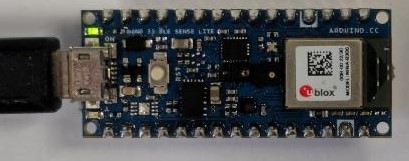
\includegraphics[width=6.5cm]{Arduino/Nano33BLE/NanoPowerLED}
    \caption{Power On Arduino Nano 33 BLE Sense}
    \label{fig:Test}
\end{figure}

\section{Testing the On-Board Sensor}

Arduino Nano 33 BLE sense have a set of on-board sensor embed on it. These sensor also start working when arduino board operate. These are the following set of sensors available in Arduino Nano 33 BLE Sense board.
\begin{itemize}
    \item The IMU is a LSM9DS1 and it is managed through I2C.
    \item The LPS22HB reads barometric pressure and environmental temperature.
    \item The HTS221 senses relative humidity.
    \item The ADPS-9960 is a digital proximity, ambient light, RGB and gesture sensor.
    \item The MP34DT05 is the digital microphone.
\end{itemize} 

\subsection{LSM9DS1 (Accelerometer, Gyroscope, and Magnetometre Sensor)}

The 9-axis inertial measurement unit (IMU) sensor is work as a accelerometre, gyroscope, and magnetic sensor. It measures 3D linear acceleration, 3D angular Velocity and 3D magnetic field aroud the sensor. This 9-axis IMU sensor use to measure Position, vibration, orientation and magnetic field around the sensor. To check the funcnality of this sensor there is avialable library in the example section as shown in the figure. \ref{fig:Testware} Go to examples check LSM9DS1 sensor, it shows all the functionality of this sensor i.e: (Accelerometer, Gyroscope, and Magnetometer).


\begin{figure}[htbp]
    \centering
    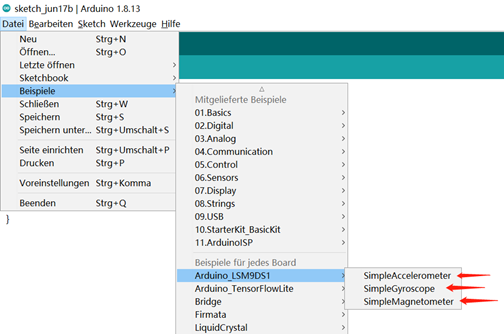
\includegraphics[width=7.5cm]{Nano33BLESense/Testware3Sensoren}
    \caption{9-Axis IMU Sensor}
    \label{fig:Testware}
\end{figure}

By getting the results and output of the 9-axis IMU sensor, first we need to upload the available library program into Arduino nano 33 BLE Sense. To avoid any trouble during uploading the program, make sure to follow all the steps as we discussed in previous chapter e.g; (choose the board, select the port during upload and change the port when need to see output in serial monitor, reset arduino when needed). By uploading the program successfully, open the serial monitor and see the result as shown in figure.\ref{fig:IMU-Test} Make sure to change the position and orientation of board and also place some Magnet aroud the borad, it shows visible changes in the output too.

\begin{figure}[htbp]
    \centering
    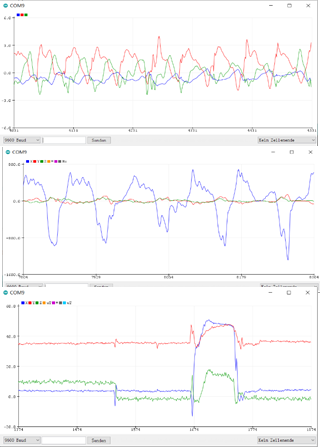
\includegraphics[width=7.5cm]{Nano33BLESense/ErgebnisseIMUTests}
    \caption{Results of IMU-Tests}
    \label{fig:IMU-Test}
\end{figure}

The above 9-Axis IMU output, shows the 3-axis values for each accelerometer, gyroscope and magnetometer. It shows how powerful the Arduino Nano 33 ble sense board and compatible with Arduino IDE the integrated development environment. These values changes as the sensor observes some changing in the sorroundings too, and it shows in the form of graph in the serial monitor. 


\bigskip

The Arduino Nano 33 BLE Sense has a built-in IMU (inertial measurement unit) that consists of two modules: the 6-axis BMI270 and the 3-axis BMM150. These modules can measure acceleration, rotation, and magnetic fields in 3D space. To use the IMU, you need to install the official Arduino library for the sensor.

Here is a simple example of how to use the IMU to read the values of the accelerometer and print them to the serial monitor:

\begin{code}
    \begin{Arduino}
        #include <Arduino_LSM9DS1.h> // include the IMU library
        
        void setup() {
            Serial.begin(9600); // initialize serial communication
            while (!Serial); // wait for serial monitor to open
            
            if (!IMU.begin()) { // initialize IMU
                Serial.println("Failed to initialize IMU!");
                while (1);
            }
        }
        
        void loop() {
            float x, y, z; // variables to store the accelerometer values
            
            if (IMU.accelerationAvailable()) { // check if new data is available
                IMU.readAcceleration(x, y, z); // read the acceleration values
                Serial.print("Acceleration x: ");
                Serial.print(x);
                Serial.print(" y: ");
                Serial.print(y);
                Serial.print(" z: ");
                Serial.println(z);
            }
        }
    \end{Arduino}
    \caption{Simple example using of the builtin IMU of the Arduino Nano 33 BLE Sense}\label{code:imu}
\end{code}

\Mynote{How to install the library PDM\\description of the lib\\ functions}





\section{Reset of the Arduino}

Due to several errors with the serial interface, it was initially assumed that the Arduino had a defect. After further tests, it turned out that the Arduino was not responsive; it had to be reset. With the help of the small button\Mynote{No?} on the Arduino board, it boots into the bootloader and can then be reloaded with a manual change of the COM port.

\begin{center}
    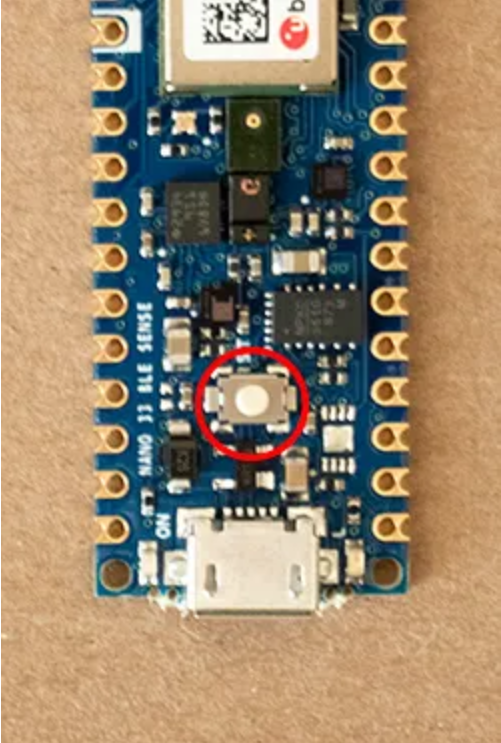
\includegraphics[width=0.4\textwidth,angle=90]{Nano33BLESense/reset.png}
    \captionof{figure}{The Reset Button of the Arduino}
\end{center}





\chapter{Testspezifikation}\label{Nano33:TestSoftware}

Ein 100\% reibungsfreier Ablauf kann nie gewährleistet werden, es können stets zufällige Fehler auftreten. Hardwareseitig kann man vor Gebrauch eine Sichtprüfung machen und die Applikation auf Schäden untersuchen. Softwareseitig ist es möglich nach dem Einschalten ein Testprogramm zu durchlaufen. 

\section{Sketch ``Hello World''}

Zur Prüfung der Entwicklungsumgebung und der grundsätzlichen Funktion der Hardware, bietet sich ein einfach Beispielsketch an, der nur eine LED ansteuert. Dieser Sketch stellt die Arduino \ac{ide} zur Verfügung. Unter dem Pfad \FILE{File/Examples/01.Basics} können kleine Beispielsketche ausgewählt werden. Hier wird das Beispiel \FILE{Fade} genutzt. Hierbei wird die eingebuate LED, welche eine RGB-LED ist, genutzt. 

\begin{Arduino}
    int brightness = 0;  // how bright the LED is
    int fadeAmount = 5;  // how many points to fade the LED by
    
    // the setup routine runs once when you press reset:
    void setup() {
        // declare LED_BUILTIN to be an output:
        pinMode(LED_BUILTIN, OUTPUT);
    }
    
    // the loop routine runs over and over again forever:
    void loop() {
        // set the brightness of LED_BUILTIN:
        analogWrite(LED_BUILTIN, brightness);
        
        // change the brightness for next time through 
        //the loop:
        brightness = brightness + fadeAmount;
        
        // reverse the direction of the fading at the ends 
        //of the fade:
        if (brightness <= 0 || brightness >= 255) {
            fadeAmount = -fadeAmount;
        }
        // wait for 30 milliseconds to see the dimming 
        //effect
        delay(30);
    }
\end{Arduino}

Als Ergebnis sollte die Helligkeit der eingebauten LED stufenweise an- und ausgehen. 


\section{Test der Sensoren eines Arduino Nano 33 BLE Sense}
	
Zur Aufgabe der Software auf dem Arduino Nano 33 BLE Sense Lite gehört das Auslesen und Übermitteln der Sensordaten an den Computer. In diesem Abschnitt erfolgt eine Beschreibung der dafür entwickelten Software.
	
\begin{Arduino}
#include <Arduino_LSM9DS1.h>  // IMU 
#include <Arduino_APDS9960.h> // Farbsensor
#include <Arduino_LPS22HB.h>  // Druck- und Temperatursensor
\end{Arduino}
	
Zu Beginn des Skriptes werden die Bibliotheken zur Ansteuerung der Sensoren eingebunden. Dafür wird der \lstinline[language=C++]|#include| Befehl verwendet.
	
\begin{Arduino}
void setup() {
  Serial.begin(9600);
  while (!Serial);
			
  // Initialisierung des Druck- und Temperatursensors
  if (!BARO.begin()) {
	Serial.println("Initialisierung des Druck- und Temperatursensor fehlgeschlagen.");
  }

  // Initialisierung der IMU
  if (!IMU.begin()) {  
	Serial.println("Initialisierung der IMU fehlgeschlagen.");   
  } 
  // Initialisierung des Farbsensors
  if(!APDS.begin()){
	Serial.println("Initialisierung des Farbsensors fehlgeschlagen.");
  }
}
\end{Arduino}
	
Zu Beginn wird einmalig die \lstinline[language=C++]|setup()| Funktion aufgerufen. Innerhalb dieser Funktionen erfolgt das Initialisieren der Bibliotheken für die jeweiligen Sensoren. Sollte eine Initialisierung fehlgeschlagen sein, liefert die Funktion \PYTHON{begin()} eine null als Rückgabewert, die zu einer eins negiert wird und es folgt die Mitteilung der fehlgeschlagenen Initialisierung an den seriellen Monitor. 
	
\begin{Arduino}
void loop() {
		int c1 = 0; // Zaehler fur Verfugbarkeitsprufung der Beschleunigungsdaten
		int c2 = 0; // Zaehler fur Verfugbarkeitsprufung der Farbsensordaten
		
		// Initialisierung der Variablen
		float x, y, z;  // IMU-Variablen
		int r, g, b;  // Farbsensor-Variablen
\end{Arduino}
	
Die Funktion \PYTHON{loop()} wird als Dauerschleife auf dem Arduino ausgeführt. Zunächst werden die Zähler für eine spätere Verfügbarkeitsprüfung der Beschleunigungs- und Farbsensordaten initialisiert. Anschließend erfolgt das Deklarieren der Variablen für das spätere Speichern der Sensordaten.
	
	\begin{Arduino}
	float druck = BARO.readPressure();        // Lesen des Drucksensors
	float temperatur = BARO.readTemperature();  // Lesen des Temperatursensors
	
	Serial.println();
	Serial.println("Testwerte des LPS22HB-Sensors:");
	Serial.println();
	// Ausgabe der gemessenen Temperatur
	Serial.print("Die Temperatur T = ");
	Serial.print(temperatur);
	Serial.println(" C wurde gemessen.");
	
	// Ausgabe des gemessenen Drucks
	Serial.print("Der Druck p = ");
	Serial.print(druck);
	Serial.println(" kPa wurde gemessen.");
	\end{Arduino}
	
	In diesem Abschnitt werden die Werte für den Druck und die Temperatur erfasst. Die \lstinline[language=C++]|BARO.readPressure()|-Funktion liefert als Rückgabewert den aktuellen Druck in kPa. Mit diesem Wert wird die Variable \lstinline[language=C++]|druck| initialisiert. Nach dem identischen Vorgehen wird die \lstinline[language=C++]|temperatur| Variable mit dem Rückgabewert der \lstinline[language=C++]|BARO.readTemperature()|-Funktion initialisiert. Anschließend erfolgt das Senden der gemessenen Information an den Port des angeschlossenen Computers.
	
	\begin{Arduino}
		// Testen der IMU
		Serial.println("Test der IMU-Einheit:");
		Serial.println();
		while (! IMU.accelerationAvailable()) {
			delay(5);
			c1++;
			if(c1 > 15)
			{
				break;
			}
		}
	\end{Arduino}
	
	Für den Test der inertialen Messeinheit wird zunächst mit einer while-Schleife \lstinline[language=C++]|while (! IMU.accelerationAvailable())| geprüft, ob die zu messenden Beschleunigungsdaten verfügbar sind. Sobald der Sensor bereit ist oder 16-mal auf die Verfügbarkeit der Sensordaten geprüft wurde \lstinline[language=C++]|if(c1 > 15)|, wird die Schleife verlassen und es folgt eine weitere Prüfung, deren Ergebnis im positiven Fall das Auslesen der Sensordaten zur Folge hat und im negativen Fall das Auslesen der Beschleunigungswerte überspringt.
	
	\begin{Arduino}
		IMU.readAcceleration(x, y, z);
		
		Serial.print("Die Beschleunigung in x-Richtung betragt ");
		Serial.print(x*100);
		Serial.println(" % der Erdbeschleunigung.");
		Serial.print("Die Beschleunigung in y-Richtung betragt ");
		Serial.print(y*100);
		Serial.println(" % der Erdbeschleunigung.");
		Serial.print("Die Beschleunigung in z-Richtung betragt ");
		Serial.print(z*100);
		Serial.println(" % der Erdbeschleunigung.");
		Serial.println();
		Serial.print("Der Betrag der addierten Beschleunigungsvektoren betragt ");
		Serial.print(sqrt(x*x+y*y+z*z)*100);
		Serial.println(" % der Erdbeschleunigung(Sollwert bei Ruhelage ca. 100 %).");
	\end{Arduino}
	
	Das Auslesen der Beschleunigungswerte erfolgt mit der \lstinline[language=C++]|IMU.readAcceleration()|-Funktion. Es wird jeweils das Verhältnis der gemessenen Beschleunigung zur herkömmlichen Erdbeschleunigung $g = 9,81 m/s^(2)$ für die drei Koordinaten-Richtungen x, y und z zurückgegeben. Zum Schluss erfolgt eine Plausibilitätsprüfung der gemessenen Werte. Dazu wird der Betrag des summierten Vektors der drei Koordinaten-Richtungen berechnet. Je nach geographischer Lage sollte der Betrag bei ca. 100 \% der Erdbeschleunigung liegen.
	
	\begin{Arduino}
		while (! APDS.colorAvailable()) {
			delay(5);
			c2++;
			if(c2 > 15)
			{
				break;
			}
		}
	\end{Arduino}
	
	Für den Farbsensor erfolgt der identische Test auf Verfügbarkeit der Sensordaten wie zuvor bei der IMU. 
	
	\begin{Arduino}
		// Auslesen der Farbwerte
		APDS.readColor(r, g, b);
		
		// Ausgeben der Farbwerte
		Serial.print("Der Rotwert r = ");
		Serial.print(r);
		Serial.println(" wurde gemessen.");
		Serial.print("Der Grunwert g = ");
		Serial.print(g);
		Serial.println(" wurde gemessen.");
		Serial.print("Der Blauwert b = ");
		Serial.print(b);
		Serial.println(" wurde gemessen.");
		Serial.println();
	\end{Arduino}
	
	Die Farbwerte für das rote, grüne und blaue Licht können mit der \lstinline[language=C++]|APDS.readColor()|-Funktion ausgelesen werden. Nach erfolgreichem Auslesen der Farbwerte werden diese an den seriellen Port gesendet.
	
	\begin{Arduino}
		// Nach 3,8 Sekunden werden die Sensordaten erneut ausgelesen.
		delay(3800);
	\end{Arduino}
	 
	 Zum Ende des vollständigen Durchlaufs der \lstinline[language=C++]|loop()|-Funktion wird das Fortschreiten des Skriptes für 3,8 Sekunden verzögert. Diese Zeit ist auf die Öffnungsdauer von vier Sekunden des seriellen Monitors auf dem Computer angepasst. In seltenen Fällen kann es dadurch zu einer doppelten Anzeige der Sensordaten in der Log-Datei kommen.


    
